\documentclass[PROP_AGutteridge_CS.tex]{subfiles}
\begin{document}

\chapter{Objectives}
The aims as outlined previously will be achieved by a comprehensive approach that both processes data and presents it in an alternative style. Figure 5 shows the proposed set of scenarios that the system will support, and that the system architecture choices will be based upon. This system will be available as a web application that is compatible with modern browsers. The key objectives are comprised of the modular components of the app, namely:
\begin{enumerate}
\item{Semantic categorisation of keywords}
\item{Geocoding of addresses}
\item{Implementation of a web framework}
\item{Visualisation of results within a web browser} 
\end{enumerate}

\begin{figure}[h!]
	\centering
	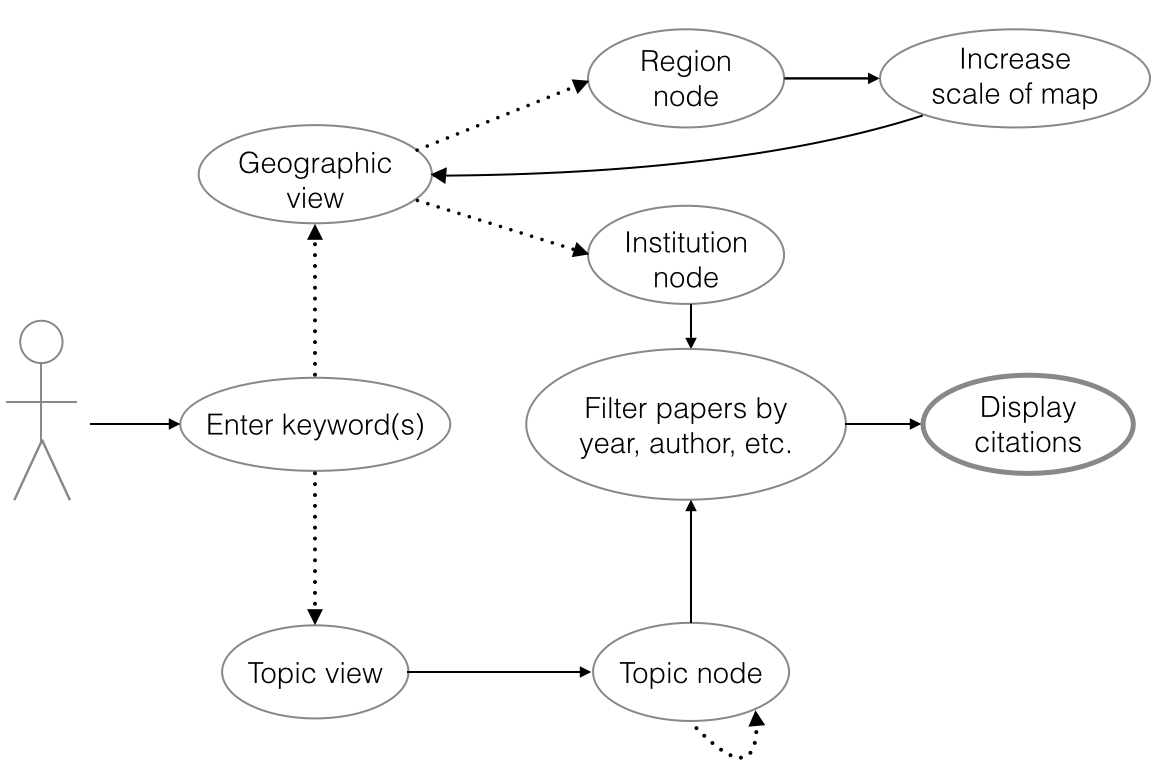
\includegraphics[width=300pt]{../lib/images/user-flowchart}
	\caption{Flowchart of the steps a user is envisioned to take when using the system. There is a single entry point to the system, as an initial query is required to retrieve data and use it to build a visualisation. This can either be viewed according to geographical locations on a world map, or as a cluster diagram categorised by subject headings. The user is then able to refine the dataset by interacting with the different nodes. When the dataset is deemed to be sufficiently specific by the user, filters can be applied in order to display a set of citations.}
\end{figure}

\noindent In order to make informed decisions on the most appropriate technologies for each aspect of the project, the listed objectives will be expanded upon in the following sections, and concluded with a set of clear deliverables and timeframes. Finally, a system architecture will be outlined that is composed of functional and compatible technologies.

\section{O1: Semantic Analysis Tools}
\subsection{MeSH terms}
Upon submission of a publication to MEDLINE, authors have the opportunity to attach MeSH terms that characterise the key concepts, biological entities and technologies of note to their work. This manual curation helps direct searches toward relevant citations and can also allow for flexibility in the specificity of terms. As seen in GoPubMed, the terms at the top levels of the hierarchy are of little use to those searching for articles of interest as they are too broad and are thus associated with a large number of citations. The proposed system will filter high-level MeSH terms out of the dataset, and group the remaining terms by the descriptor types. MeSH 2015 has 16 categories\cite{mesh2015} that are organised into tree-like structures, an example of which is shown in Figure 6. The vocabulary is free to download in full, formatted as either XML or ASCII text. A server-side database system is proposed has been utilised in previous works\cite{stoyanovich}. As synonyms are represented in each record by a list of unique identifiers, each of which in itself representing a record, a relational database with unique identifiers as the primary key would be the most efficient method of preserving and utilising these connections. 

\begin{figure}[ht]
	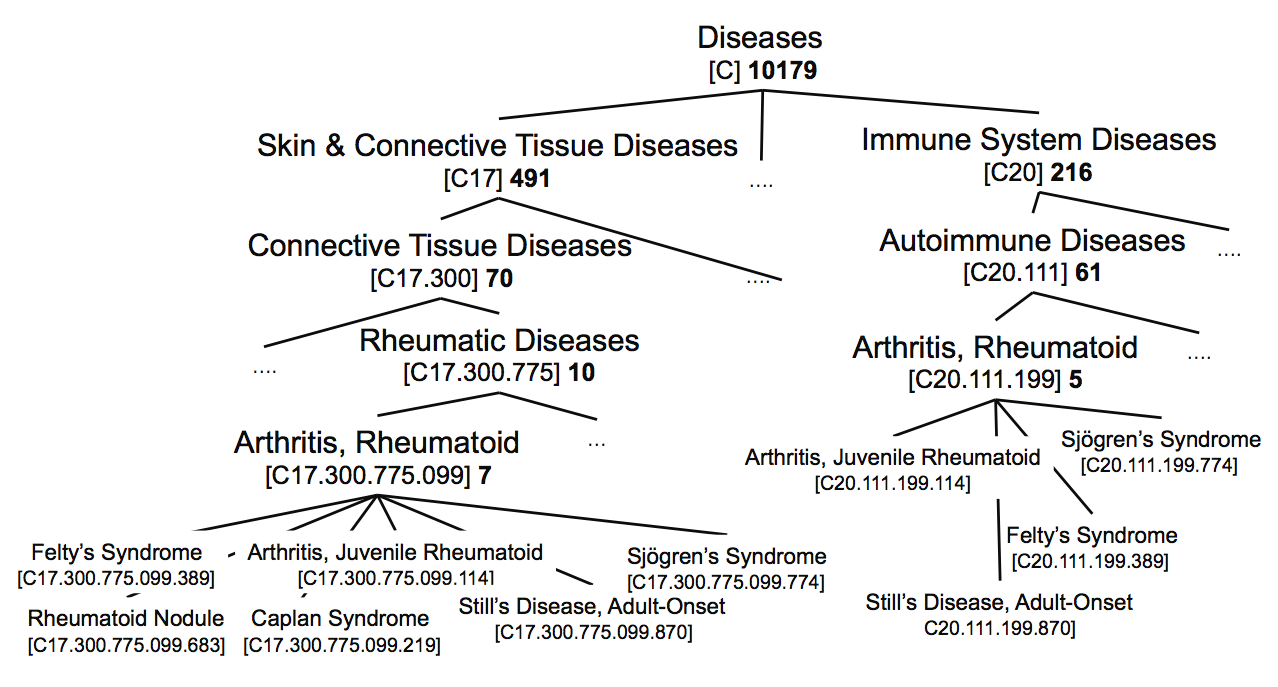
\includegraphics[width=\textwidth]{../lib/images/MeSH}
	\caption{Sample of the hierarchical structure of MeSH terms, centred around rheumatoid arthritis. Each node has a tree number for fast search Taken from \cite{stoyanovich}.}
\end{figure}
	
\subsection{Author keywords}
Due to the dependency of MeSH terms on human time and energy, the coverage of the PubMed database is not comprehensive. Many publications provide keywords that are suggested by the authors alongside the manuscript. The challenge here is that these words do not follow the MeSH vocabulary, and are therefore more likely to be variable, producing datasets that are difficult to group efficiently. Additionally, the specificity of the word is not known; the term may denote a high-level concept (e.g. mammal) or may be extremely specific (e.g. MPTP mouse, an animal model of Parkinson's Disease). Fortunately, unlike MeSH terms, high-level tags are not enforced upon papers so it is largely expected that keywords will be relevant to the topics explored within the publication. Initially, author keywords will be compared to the MeSH vocabulary to see if an exact match can be found. If there is no direct map to a MeSH term, the phrase will be presented as a potential new term--appearing in a node of its own. A threshold number of citations will be established to prevent creation of noisy datasets that contain a large number of single-citation nodes. 

\subsection{MetaMap}
The National Library of Medicine has integrated MeSH and a number of other vocabularies and tools to produce a comprehensive set of services termed the Unified Medical Language System (UMLS)\cite{bodenreider}. The most relevant tools for this project are Metathesaurus, a database of BioMedical vocabularies, and MetaMap, a Prolog-based mapping engine\cite{aronson}. In addition to the greater number of concepts and relationships characterised by the UMLS, a higher degree of semantic annotation is accessible when compared with the MeSH knowledge base. Ambiguities between unrelated terms are represented, and the relationship between concepts are stored as verbs such as \emph{treats, contains,} and \emph{causes}. Much of this information is beyond the scope of this project, however it would be simpler to process MeSH terms and author keywords using the same pipeline, and would likely result in a richer dataset with which to produce a visualisation. The technical disadvantage of using the UMLS lies in the access of data via MetaMap. The program is large at 7 GB, and 2 GB of memory is recommended. These requirements are likely too strenuous for an inexpensive server. Alternatively, the Java API provides access the mapping engine, the output of which could be parsed as JSON or XML and sent to the web framework as a response. There is a Clojure wrapper for the 2013v2 API release, which I would be interested in using as I have basic knowledge of Racket, another Lisp dialect language. 

\subsection{O1: Deliverables}
There are two clear alternatives for semantic processing of BioMedical keywords, the investigation into which should be carried out early on in the project as it will affect the system architecture. The key milestones in objective 1 are:
\begin{enumerate}
\item{Install MetaMap Java API, investigate speed and format of output - 3--7 days}
If this approach does not appear appropriate:
\item{Investigate relational database solutions - 1--2 days}
\item{Download MeSH XML file and enter a small number of records into database - 2--4 days}
\end{enumerate}

\noindent At this stage in the project development of the web framework should begin to ensure that all components are compatible. 

\section{O2: Geocoding of Addresses}
\subsection{Map Technologies}
The geographic view relies on the presentation of the world map in a scalable format. Google Maps (\url{UK, http://maps.google.co.uk/}) and OpenStreetMap (OSM, \url{http://openstreetmap.org/}) are both widely used in both desktop and mobile web applications. OpenStreetMap is initially more appealing, as it is open-source and customisable with alternative tilesets. However, the main feature of interest is the ability of the map service to interpret an address string and return a geographical location, termed \emph{geocoding}. Upon investigation of searching for institutional addresses on both services, Google was the clear winner (see Appendix Table 1). The poor coverage of China by OSM may be due to the Surveying and Mapping Law of the People's Republic of China\cite{maplaw}, and is an important factor in mapping of organisations as a large number of papers are published by Chinese researchers. The Google Places API returns either JSON or XML data in response to sending a HTTP request containing a search string. Since this requires little processing, the requests will probably be made client-side after normalising the address server-side. Unfortunately, the terms and conditions of using the API state that the results must be displayed on Google Maps.

\subsection{O2: Deliverables}
The key milestones in objective 2 are:
\begin{enumerate}
\item{Write script to optimise address strings for the Google Places API - 1--2 weeks}
\item{Ensure that Google Maps can be embedded in the web page - 1--2 days}
\end{enumerate}

\section{Programming Languages and Web frameworks}
\subsection{Python vs. Ruby}
NCBI allows public access to the Entrez databases via the E-utilities (or eUtils) API, which follows a RESTful architecture structure. Sending HTTP requests can be easily achieved in a variety of programming languages. I have chosen to focus on dynamic programming languages as these allow for fast iterative development, which is particularly useful for web applications. I am familiar with Python and Ruby, and each have a multitude of full-stack frameworks and microframeworks to choose from. Python provides comprehensive functionality with modules for sending HTTP requests (urllib and httplib in Python 2, or urllib.request/urllib.parse/urllib.error and http.client in Python 3) and parsing XML (xml.etree.ElementTree) in the standard library. Ruby has modules for HTTP requests, but XML handling requires additional software. Despite having basic knowledge of Ruby, I am keen to learn Python and feel that overall, it is better suited for the task.

\subsection{Flask vs. Bottle}
At this stage of the project I am unsure of the requirement for large-scale persistence of data, in which case it may be best to go forward with a microframework. This will allow for flexibility when evaluating database technologies throughout development, as full-stack frameworks such as Django require a database engine for certain features. Two microframeworks of interest are Flask (\url{http://flask.pocoo.org/}) and Bottle (\url{http://bottlepy.org/}), both of which are lightweight, supportive of RESTful APIs, and well-documented. Considering that this project is my first experience in web development, extensive documentation is a priority for choosing a framework, and an active community is also preferred. Searching for questions tagged with 'bottle' or 'flask' on StackOverflow produced 786 and 7,387 results, respectively, indicating that Flask is more popular and thus will be better supported on forums and other online communities. For this reason Flask is chosen as the most appropriate microframework with which to build the server-side of the application.

\subsection{O3: Deliverables}
The key milestones in objective ?: implementation of a web framework, are:
\begin{enumerate}
\item{Create skeleton server-side application using Flask - 1--2 days} 
\item{Fetch data from the PubMed database - 1--3 days}
\item{Parse XML/JSON to create Objects from citation data - 1--3 days}
\item{Write basic CSS and HTML for front-end - 1--2 weeks}
\end{enumerate}

% The estimated timeframe for this objective is 10 days -- 3 weeks and 1 day.

\section{Visualisation Libraries}
\subsection{Why JavaScript?} 

\subsection{D3 vs. ???}

\subsection{O4: Deliverables}

\section{Proposed System Architecture and Usage}
The outline of the system as proposed in the objectives can be organised to create a web application with a server-side for retrieval and processing of results from PubMed, and a client-side for visualisation of the results. This is shown as a diagram in Figure 4. Figure 5 shows the proposed set of scenarios that the system will support in the form of a flowchart. These two diagrams together will influence the system architecture choices to fulfil the goals of implementing these features both server-side and client-side. Each of the listed objectives will be expanded upon in the following sections, and concluded with a set of clear deliverables and timeframes. 

\sidecaptionvpos{figure}{t} %trailing?
\begin{SCfigure}[][h]
 	\caption{High-level diagram of the structure of and interaction between architecture components. 1. The user interacts with the web application. 2. This sends the query to the server, 3. which sends a GET request to the PubMed database and retrieves the results in XML or JSON format, 4/5. These two stages are interchangeable, as they are concerned with different type of data. Keyword processing will be carried out on the fields holding MeSH term and author keywords using a locally stored knowledge base. Address disambiguation will use an external service to associate organisation addresses with geographical locations. 6. The processed data is sent client-side and 7. is visualised in the web browser.}
	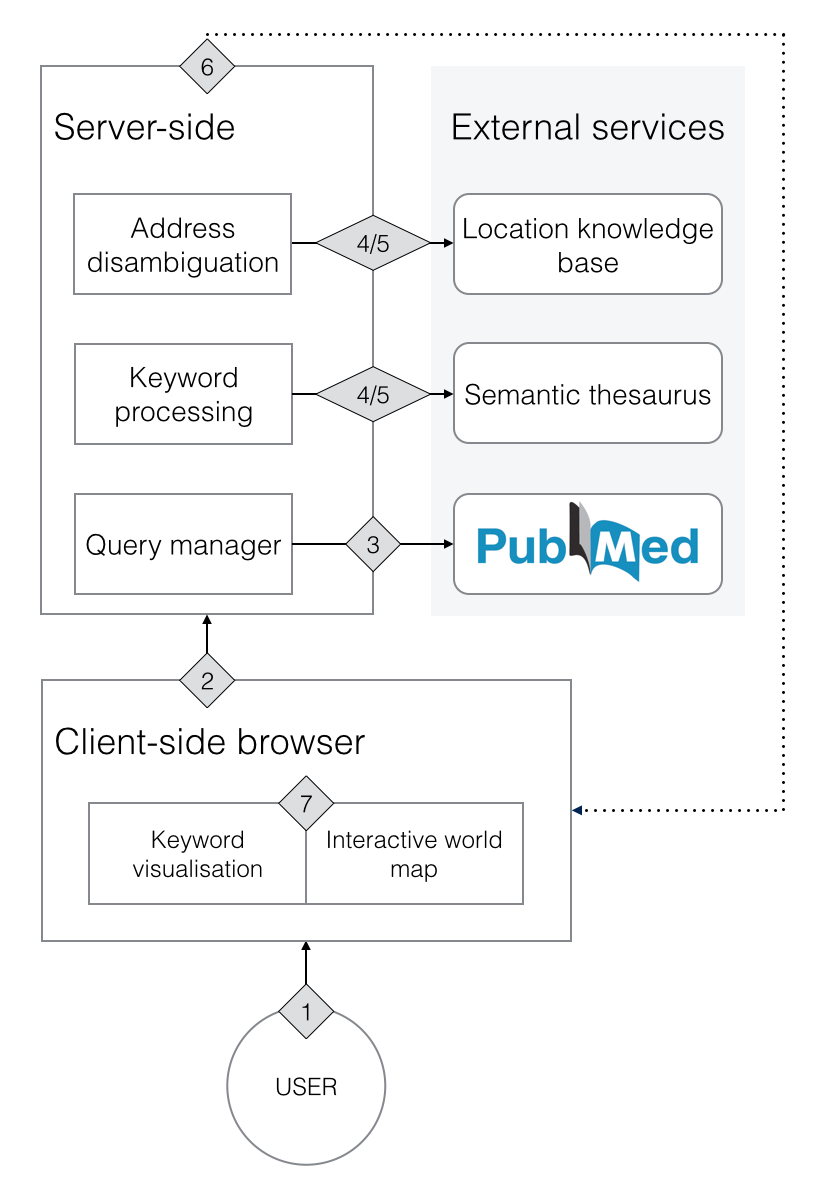
\includegraphics{../lib/images/system-arch}
	\label{fig:SA}
\end{SCfigure}

% wrap up this section! just go on to say okay all cool, now work plan?

\end{document}